\documentclass{pssbmac}

%%%%%%%%%%%%%%%%%%%%%%%%%%%%%%%%%%%%%%%%%%%%%%%%%%%%%%%%%%%%%%%%%%%%%%%%
%% POR FAVOR, NÃO FAÇA MUDANÇAS NESSE PADRÃO QUE ACARRETEM  EM
%% ALTERAÇÃO NA FORMATAÇÃO FINAL DO TEXTO
%%%%%%%%%%%%%%%%%%%%%%%%%%%%%%%%%%%%%%%%%%%%%%%%%%%%%%%%%%%%%%%%%%%%%%%%

%%%%%%%%%%%%%%%%%%%%%%%%%%%%%%%%%%%%%%%%%%%%%%%%%%%%%%%%%%%%%%%%%%%%%%%%
% POR FAVOR, ESCOLHA CONFORME O CASO
%%%%%%%%%%%%%%%%%%%%%%%%%%%%%%%%%%%%%%%%%%%%%%%%%%%%%%%%%%%%%%%%%%%%%%%%
\usepackage[brazil]{babel} % texto em Português
%\usepackage[english]{babel} % texto em Inglês

%\usepackage[latin1]{inputenc} % acentuação em Português ISO-8859-1
\usepackage[utf8]{inputenc} % acentuação em Português UTF-8
%%%%%%%%%%%%%%%%%%%%%%%%%%%%%%%%%%%%%%%%%%%%%%%%%%%%%%%%%%%%%%%%%%%%%%%%


%%%%%%%%%%%%%%%%%%%%%%%%%%%%%%%%%%%%%%%%%%%%%%%%%%%%%%%%%%%%%%%%%%%%%%%%
%% POR FAVOR, NÃO ALTERAR
%%%%%%%%%%%%%%%%%%%%%%%%%%%%%%%%%%%%%%%%%%%%%%%%%%%%%%%%%%%%%%%%%%%%%%%%
\usepackage[T1]{fontenc}
\usepackage{float}
\usepackage{graphics}
\usepackage{graphicx}
\usepackage{epsfig}
\usepackage{indentfirst}
\usepackage{amsmath, amsfonts, amssymb, amsthm}
\usepackage{url}
\usepackage{csquotes}
% Ambientes pré-definidos
\newtheorem{theorem}{Theorem}[section]
\newtheorem{lemma}{Lemma}[section]
\newtheorem{proposition}{Proposition}[section]
\newtheorem{definition}{Definition}[section]
\newtheorem{remark}{Remark}[section]
\newtheorem{corollary}{Corollary}[section]
\newtheorem{teorema}{Teorema}[section]
\newtheorem{lema}{Lema}[section]
\newtheorem{prop}{Proposi\c{c}\~ao}[section]
\newtheorem{defi}{Defini\c{c}\~ao}[section]
\newtheorem{obs}{Observa\c{c}\~ao}[section]
\newtheorem{cor}{Corol\'ario}[section]

% ref bibliográficas
\usepackage[backend=biber, style=numeric-comp, maxnames=50]{biblatex}
\addbibresource{refs.bib}
\DeclareTextFontCommand{\emph}{\boldmath\bfseries}
\DefineBibliographyStrings{brazil}{phdthesis = {Tese de doutorado}}
\DefineBibliographyStrings{brazil}{mathesis = {Disserta\c{c}\~{a}o de mestrado}}
\DefineBibliographyStrings{english}{mathesis = {Master dissertation}}
%%%%%%%%%%%%%%%%%%%%%%%%%%%%%%%%%%%%%%%%%%%%%%%%%%%%%%%%%%%%%%%%%%%%%%%%


\begin{document}

%%%%%%%%%%%%%%%%%%%%%%%%%%%%%%%%%%%%%%%%%%%%%%%%%%%%%%%%%%%%%%%%%%%%%%%%
% TÍTULO E AUTORAS(ES)
%%%%%%%%%%%%%%%%%%%%%%%%%%%%%%%%%%%%%%%%%%%%%%%%%%%%%%%%%%%%%%%%%%%%%%%%

\title{Uma comparação do paradigma funcional e iterativo na programação de Métodos Numéricos}

\author{
{\large Pazini, D. S.}\thanks{danieldspazini3@gmail.com}\\
{\large D'Afonseca, L. A.}\thanks{autor2@email}  \\
{\large Rocha, L. M.}\thanks{autor3@email}  \\
{\small DM/CEFET-MG, Belo Horizonte, MG} \\
}
\criartitulo
%%%%%%%%%%%%%%%%%%%%%%%%%%%%%%%%%%%%%%%%%%%%%%%%%%%%%%%%%%%%%%%%%%%%%%%%


%%%%%%%%%%%%%%%%%%%%%%%%%%%%%%%%%%%%%%%%%%%%%%%%%%%%%%%%%%%%%%%%%%%%%%%%
% TEXTO
%%%%%%%%%%%%%%%%%%%%%%%%%%%%%%%%%%%%%%%%%%%%%%%%%%%%%%%%%%%%%%%%%%%%%%%%

Este trabalho mostra como a programação em uma linguagem funcional, como Haskell, é muito mais natural para matemáticos que no paradigma imperativo, tomando C de exemplo, comparando a implementação do método de Newton-Raphson para busca de zeros de funções reais em ambas abordagens.

O método de Newton-Raphson é um caso particular do método do ponto fixo, que substitui o problema de encontrar zeros de uma função $f$ pela procura dos pontos fixos de uma outra função $\varphi$ chamada \textit{função de iteração de ponto fixo} construída a partir desta isolando $x$ na equação $f(x) = 0$, o que pode ser obtido de várias formas, sendo no método trabalhado o caso no qual 

\begin{equation}
    \varphi(x) = x - \frac{f(x)}{f'(x)}\label{mnr}
\end{equation}

sendo usada tal função para construção de uma sequência iterativa onde $x_k = \varphi(x_{k-1})$.~\cite{Vera}

\begin{figure}[H]
    \centering
    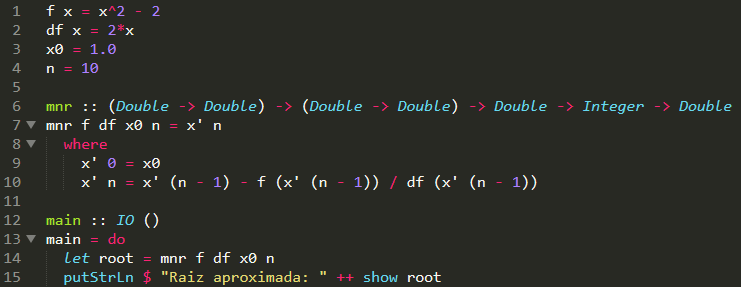
\includegraphics[width=.75\textwidth]{images/haskell.png}
    \caption{ {\small Implementação do Método de Newthon-Raphson em Haskell. Fonte: Autor.}}
    \label{fig:haskell}
\end{figure}

\begin{figure}[H]
    \centering
    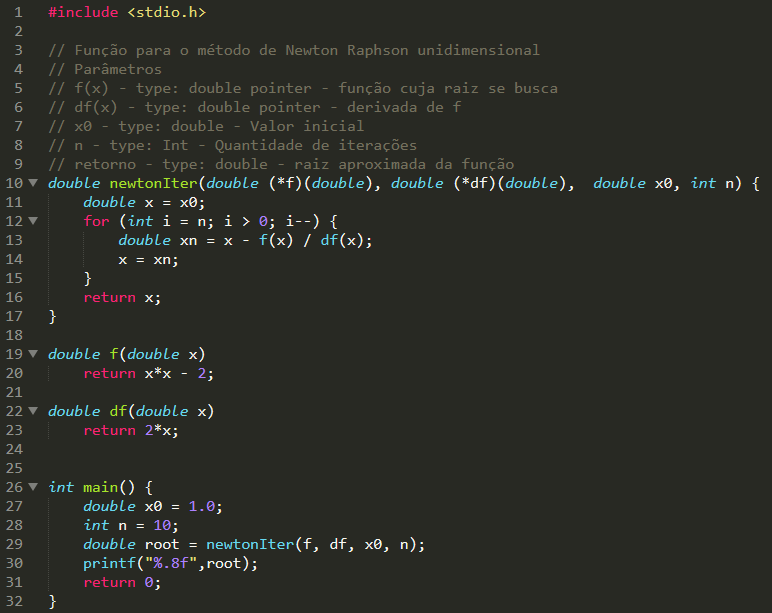
\includegraphics[width=.75\textwidth]{images/c.png}
    \caption{ {\small Implementação do Método de Newthon-Raphson em C. Fonte: Autor.}}
    \label{fig:c}
\end{figure}

É possível perceber a concisão e clareza do paradigma funcional, que inclusive recebe esse nome por ser baseado no conceito de funções matemáticas, o que explica a concisão e clareza perceptíveis no Haskell em comparação com o C. 

Em programação funcional, em distinção da imperativa, = não é um sinal de atribuição mas uma definição de uma função com seus elementos do dominío tendo valor fixo na avaliação. Além disso, a natureza recursiva do método iterativo de Newton-Raphson é ideal para programação funcional que utiliza de recursões para avaliação ao invés de iterações e sequenciamento, o que permite ficar explícita a sua forma matemática e iterativa.

\section*{Agradecimentos}
Lucas pela paciência, bom humor e orientação; Enzo por ser um dupla excepcional; D'Afonseca pelo amparo matemático e pela bolsa; a família por me proporcionar a possibilidade de chegar até aqui; a Deus; a minha querida Jaque por toda motivação.


%%%%%%%%%%%%%%%%%%%%%%%%%%%%%%%%%%%%%%%%%%%%%%%%%%%%%%%%%%%%%%%%%%%%%%%%
% REFS BIBLIOGRÁFICAS
% POR FAVOR, NÃO ALTERAR
%%%%%%%%%%%%%%%%%%%%%%%%%%%%%%%%%%%%%%%%%%%%%%%%%%%%%%%%%%%%%%%%%%%%%%%%
\printbibliography
%%%%%%%%%%%%%%%%%%%%%%%%%%%%%%%%%%%%%%%%%%%%%%%%%%%%%%%%%%%%%%%%%%%%%%%%

\end{document}




